\begin{mainquestion}{superposition}{Your Turn}
Consider the circuit below:

\begin{center}
    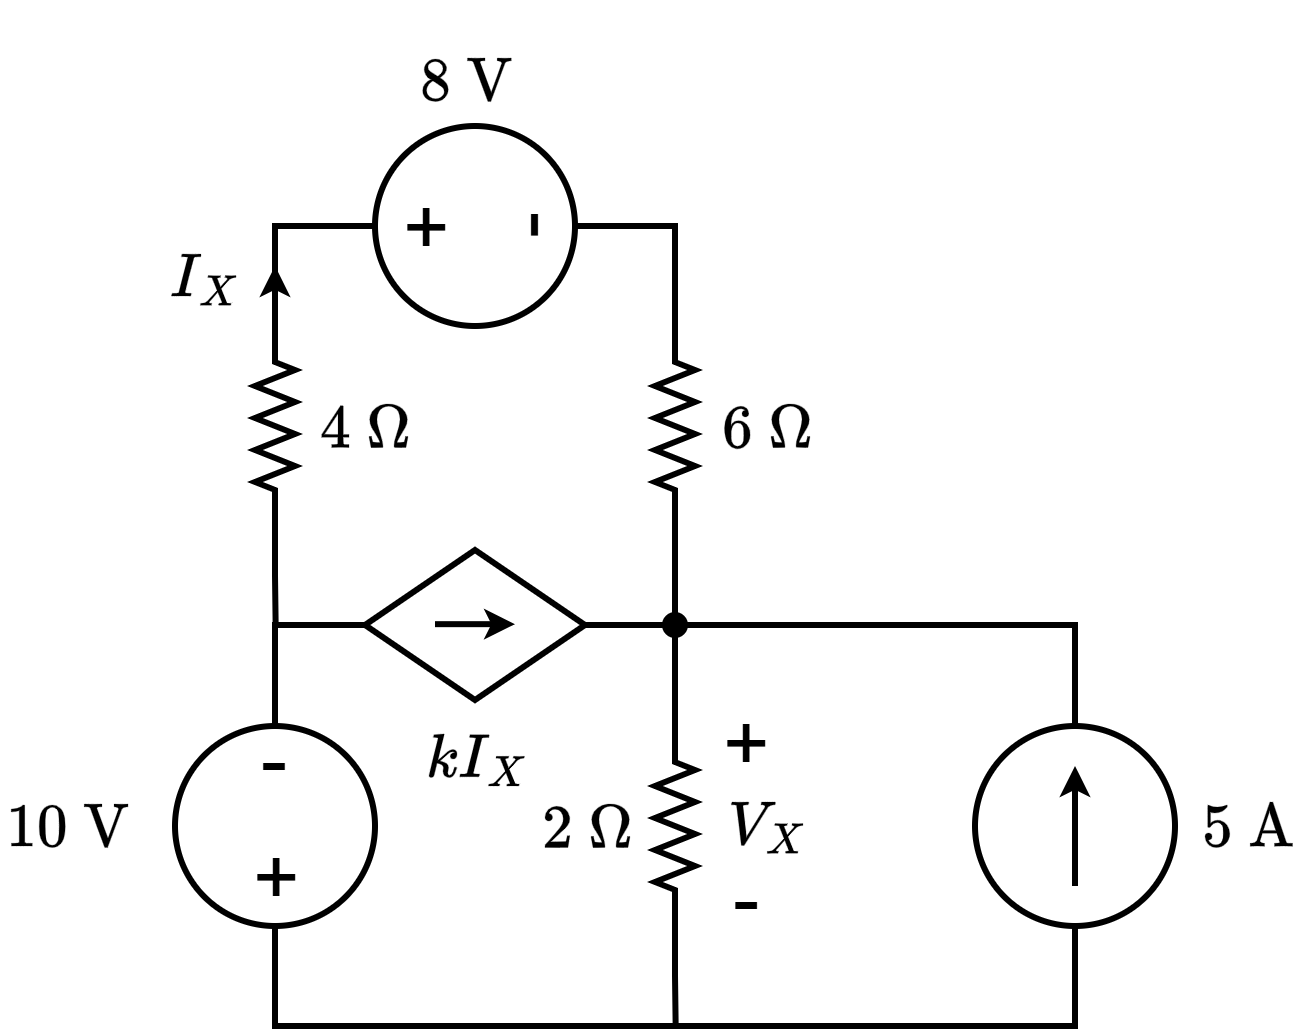
\includegraphics[width=0.8\textwidth]{super_cir.png}
\end{center}

\begin{partquestion}{calculatevx}{Given the current gain $k = 0.25$, use superposition to determine $V_X$.}
\begin{answer}
Superposition tells us that we can consider the effect of each independent source individually. We can do this by disabling all but one of the independent sources (open current sources, short voltage sources) and solving for $V_X$. Keep in mind you shouldn't deactivate any dependent sources. Then we can add up all the results and we should get the final value of $V_X$.
\bigskip

\textbf{5 A source only:} short the 10 V and 8V sources. The \qty{4}{\ohm} and \qty{6}{\ohm} resistors can be combined and the whole circuit can be redrawn to look like a current divider as seen below:
\begin{center}
    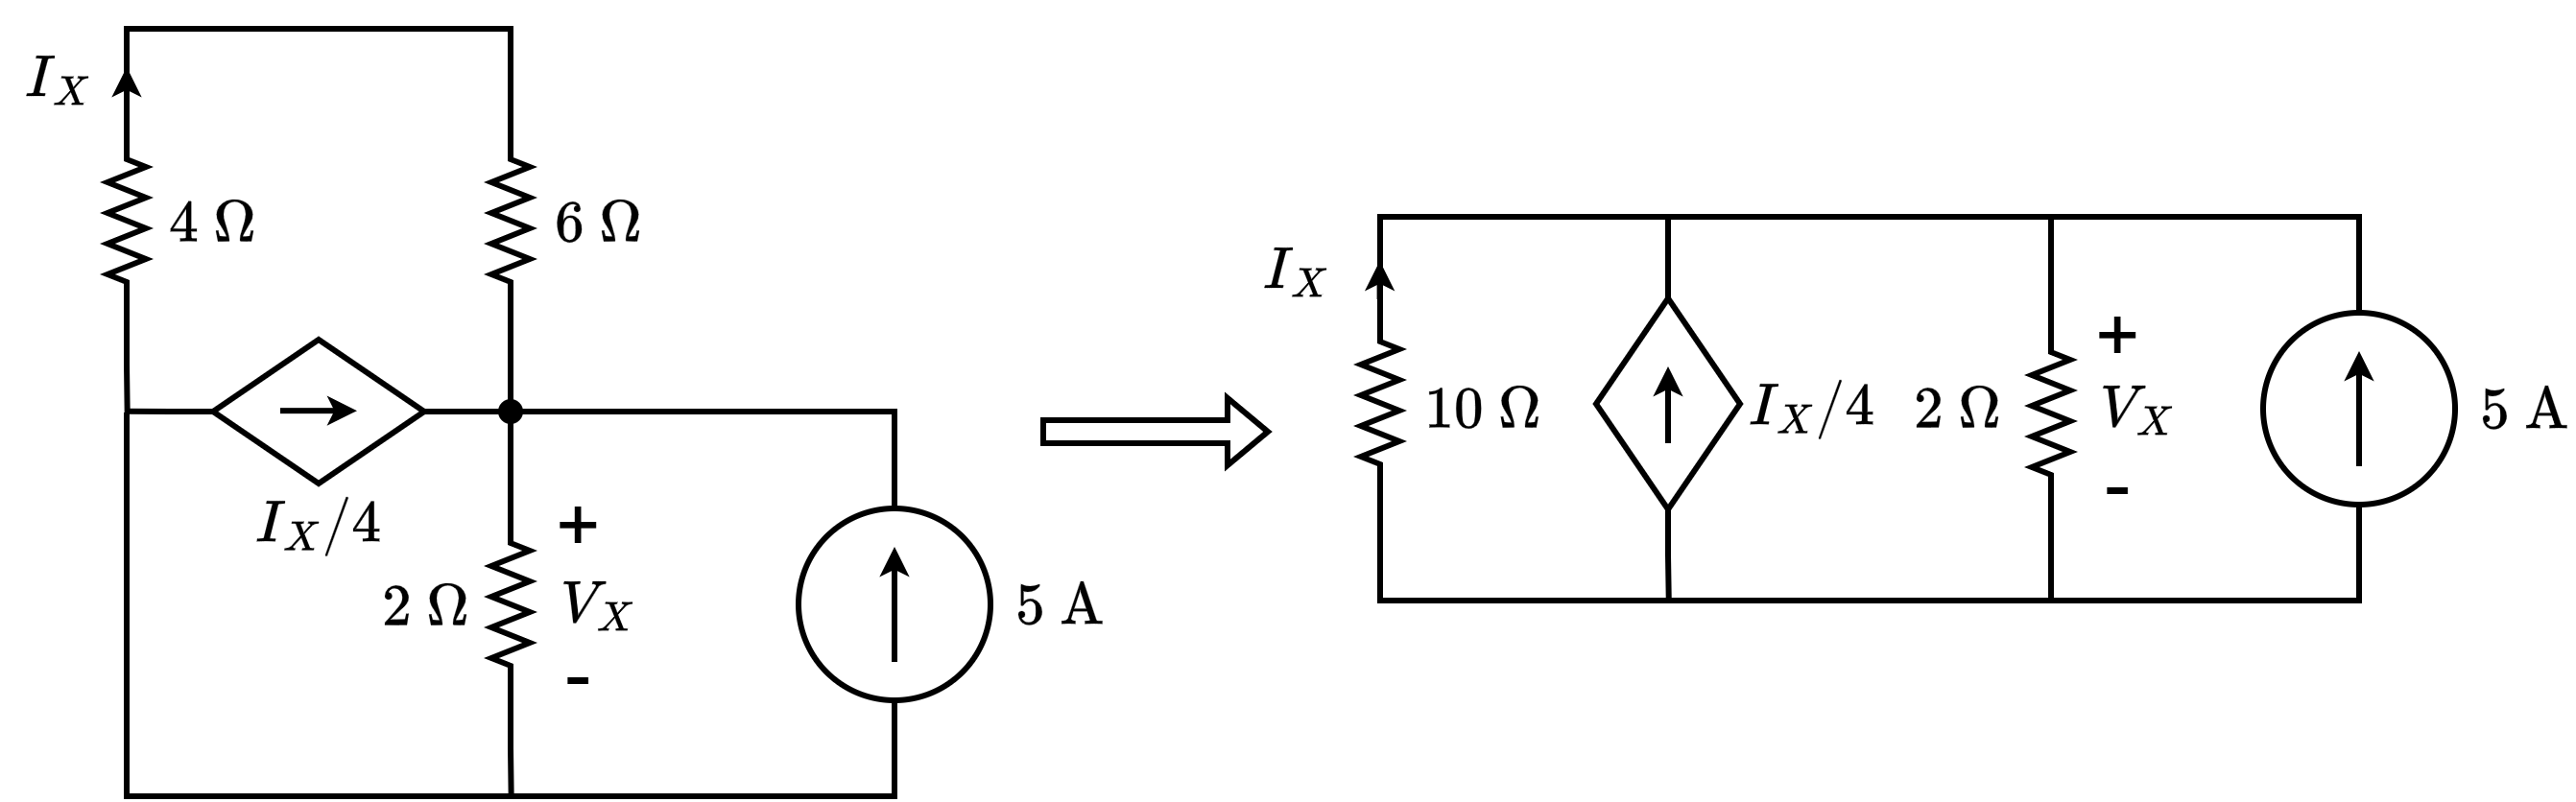
\includegraphics[width=0.9\textwidth]{super_5A.png}
\end{center}

KCL at the top node gives $5 = V_X/2 - I_X - I_X/4$. $I_X$ can be found with ohms law as $I_X = -V_X/10$. Substituting yields:
\begin{gather*}
5 = \frac{V_X}{2} - I_X\frac{5}{4} \\
5 = \frac{V_X}{2} + \frac{V_X}{8} \\
V_X = \frac{5}{\frac{1}{2}+\frac{1}{8}} = \qty{8}{\volt}
\end{gather*}
Thus $V_X = 8~\text{V}$ due to the 5 A current source.
\bigskip

\textbf{8 V source only:} open the 5 A source and short the 10 V source. Combine the resistors as before and the circuit can be rewritten as follows:
\begin{center}
    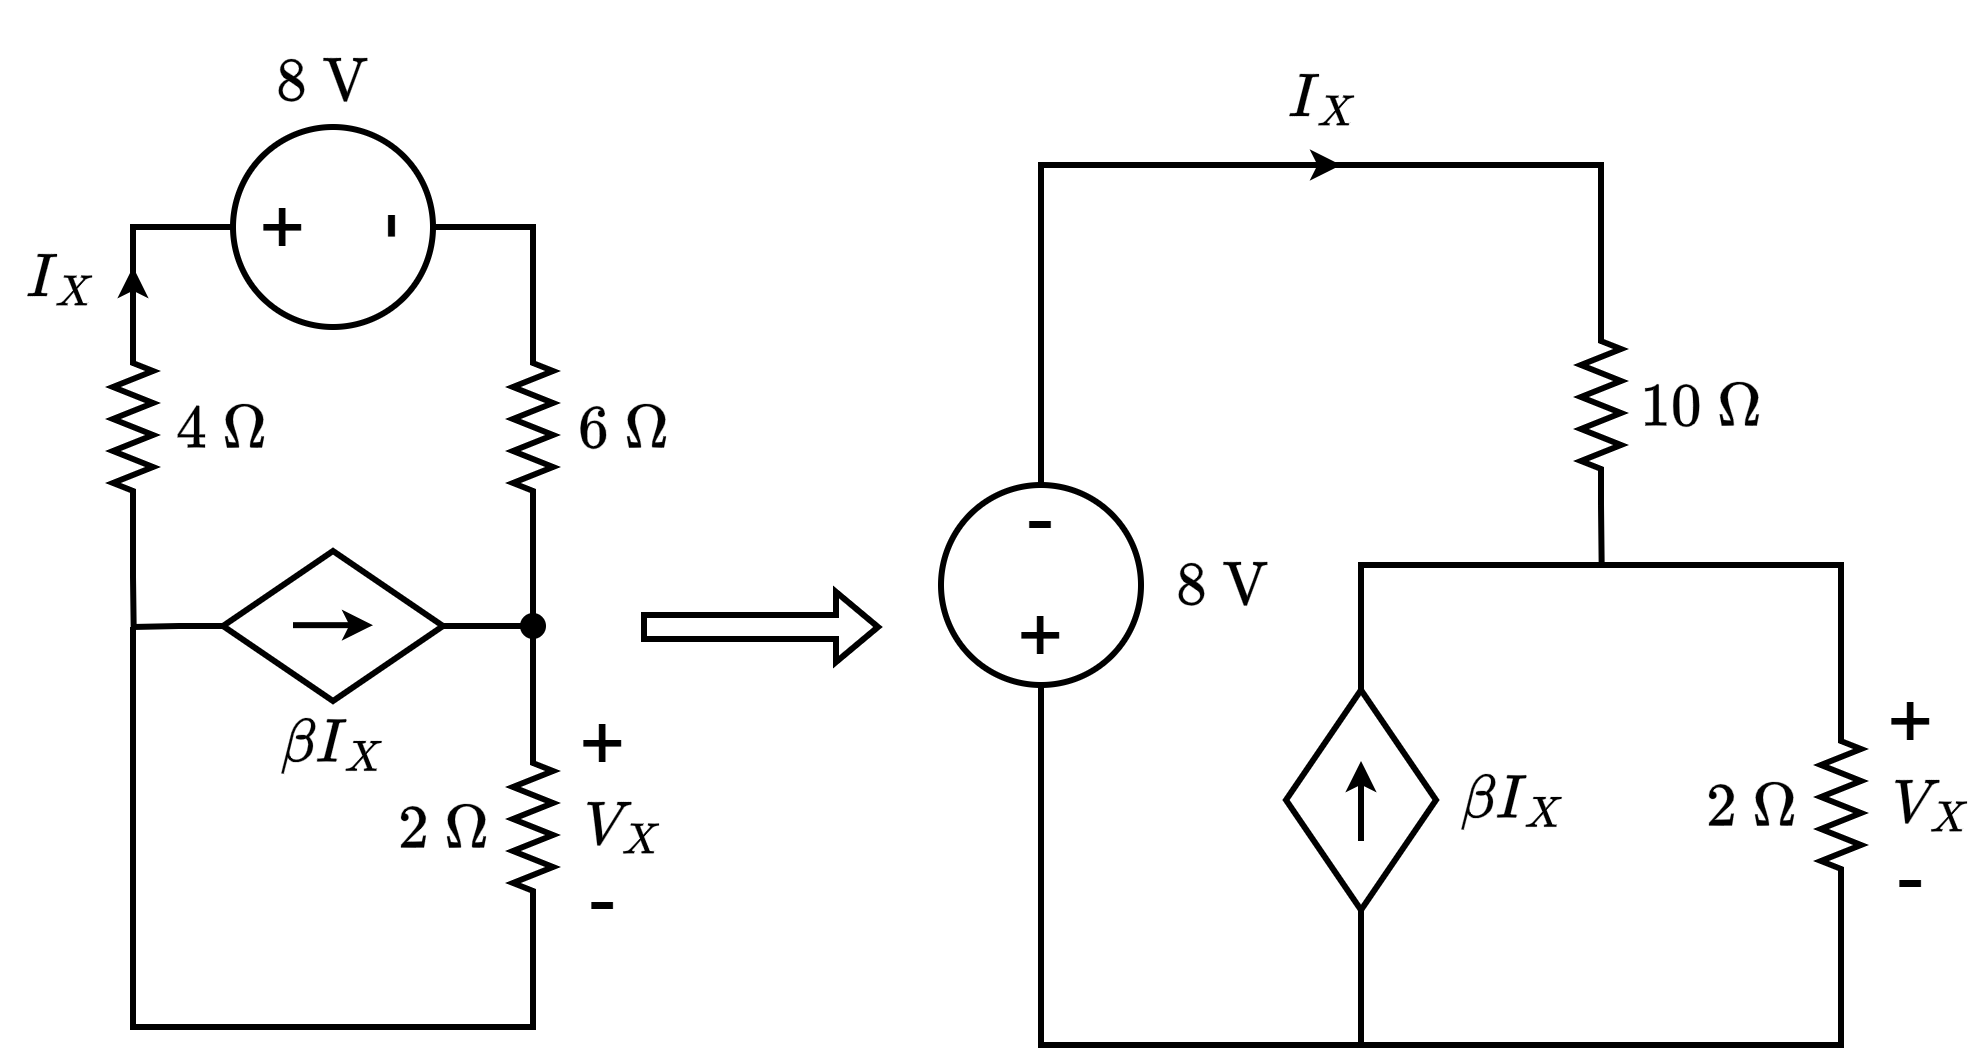
\includegraphics[width=0.9\textwidth]{../v1/super_8V.png}
\end{center}

 This could be solved as before using a KCL equation at the top of the \qty{2}{\ohm} resistor: \[\frac{V_X}{2} - I_X - \frac{I_X}{4} = 0 \hspace{1cm} I_X = \frac{-8 - V_X}{10}\]
 Solving...
\begin{gather*}
\frac{V_X}{2} - I_X\frac{5}{4}= 0 \\
\frac{V_X}{2} - \frac{(-8 - V_X)}{10}\frac{5}{4}= 0 \\
V_X\left(\frac{1}{2} + \frac{1}{8}\right) = -1 \\
V_X = -\frac{8}{5}\unit{\volt}
\end{gather*}
Thus $V_X = -\frac{8}{5}~\text{V}$ due to the 8 V voltage source.
\bigskip

\textbf{10 V source only:} open the 5 A source and short the 8 V source. Combine the resistors as before and the circuit can be rewritten as follows:
\begin{center}
    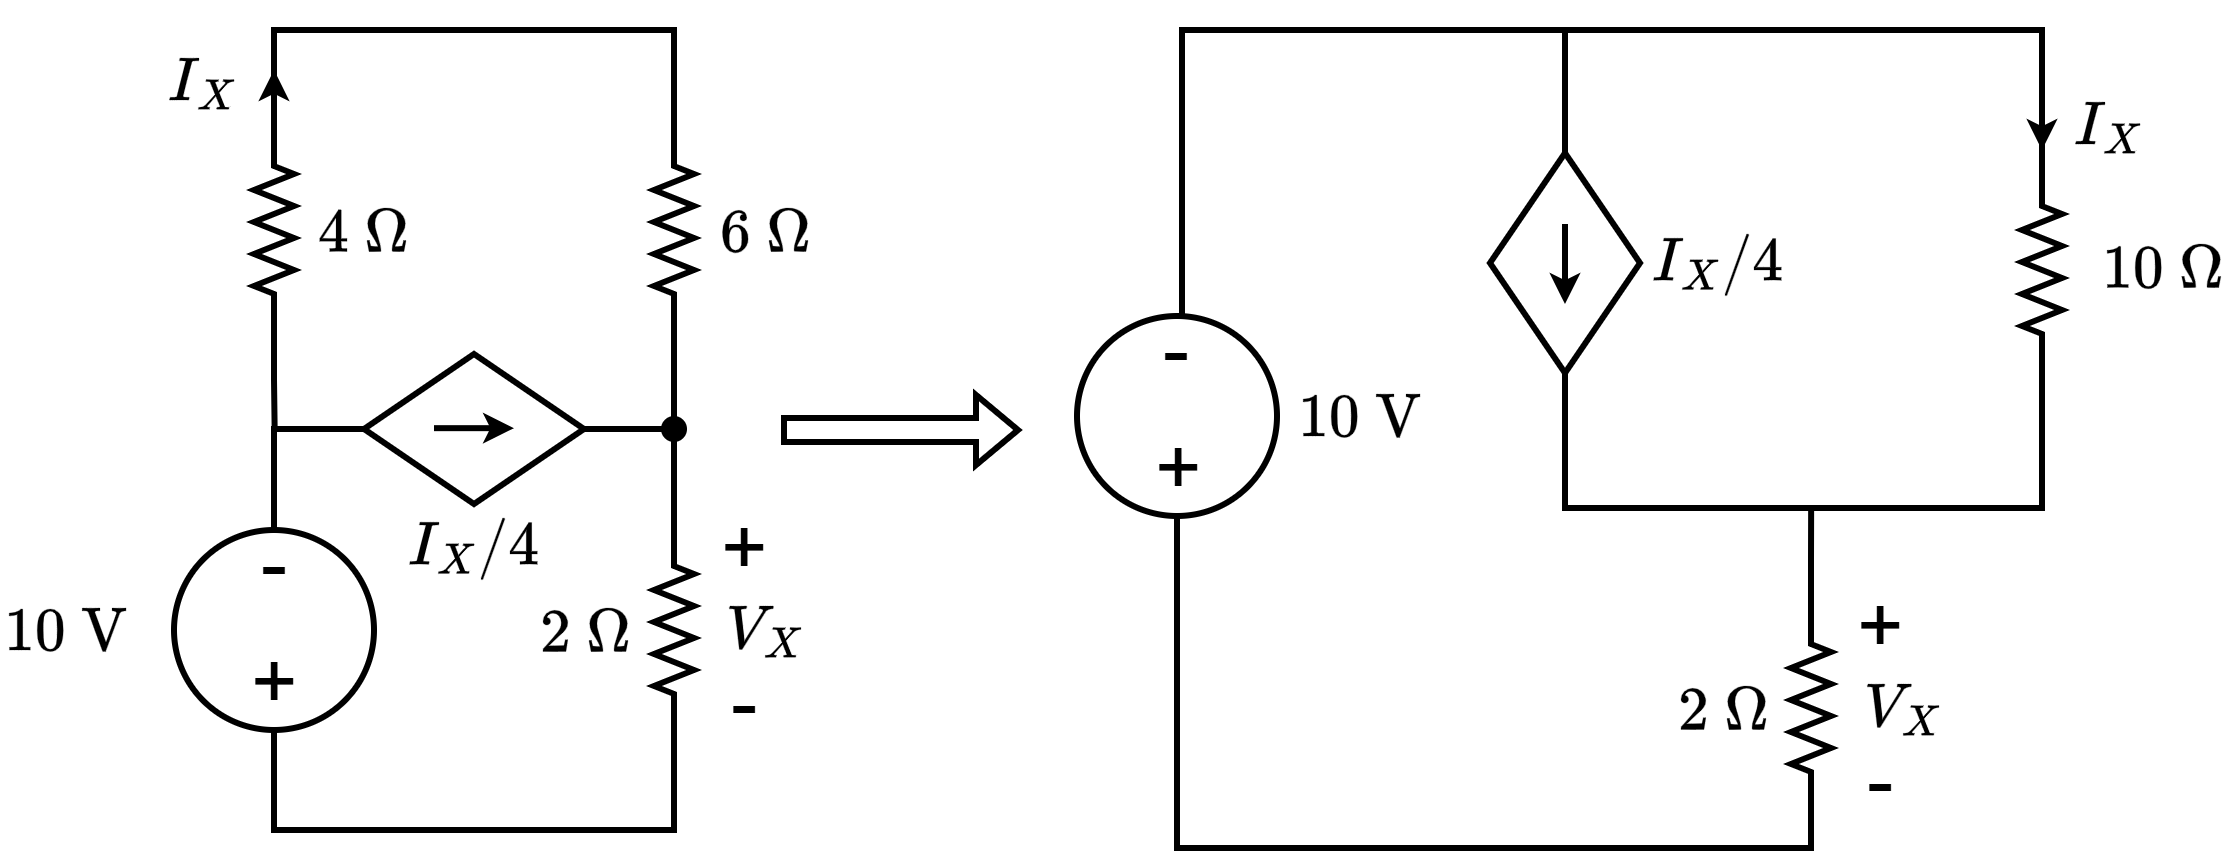
\includegraphics[width=0.9\textwidth]{super_10V.png}
\end{center}

 This could be solved as before using a KCL equation at the top of the \qty{2}{\ohm} resistor: \[\frac{V_X}{2} + I_X + \frac{I_X}{4} = 0 \hspace{1cm} I_X = \frac{-10 - V_X}{10}\]

 Another clever method would be to recognize that the current source can be modeled as a resistor. Note that the current through the dependent branch is proportional to the \qty{10}{\ohm} resistor which shares the same votlage. Since the current through the element is proportional to its  own voltage, we can use Ohm's law to describe it. Let's call the voltage across these resistors $V_A$ and note $I_X = V_A/10$:

 \[R_{\text{source}} = \frac{V_A}{I_X/4} = \frac{V_A}{{V_A}/(10\cdot4)} = \qty{40}{\ohm}\]

We can now use this resistor value to solve the voltage divider. First note that \qty{40}{\ohm} in parallel with \qty{10}{\ohm} is $\frac{40\cdot10}{40+10} = 8\unit{\ohm}$. Plugging this into the voltage divider equations yields:

\[
V_X = V_S\frac{R_{\text{bot}}}{R_{\text{bot}} + R_{\text{top}}} = -10\frac{2}{2 + 8} = \qty{-2}{\volt}
\]
 
\textbf{Summation:}

Superposition sums all the contributions:
\[
V_X = 8 - \frac{8}{5} - 2 = \frac{22}{5} = \qty{4.4}{\volt}
\]
\end{answer}
\end{partquestion}

\begin{partquestion}{verifysuper}{Find $k$ such that $V_X = \qty{17}{\volt}$}
\end{partquestion}

\end{mainquestion}
